\documentclass{article}
\usepackage[utf8]{inputenc}
\usepackage{graphicx}
\usepackage{fullpage}
\usepackage{rotating}


\title{LINGI2261 : Artificial Intelligence \\ Assigment 2: Solving Problems with Informed Search}
\author{Alexandre Hauet \& Tanguy Vassen \\ Group 21}
\date{October 2015} 

\begin{document}

\maketitle


\section{$A^{*}$ versus uniform-cost search}

\subsection*{Give a consistent heuristic for this problem. Prove it is admissible.}
Manhattan distance between the man and the euro is a nice heuristic to solve this kind of problem. Theoretically, manhattan distance give us always the shortest distance. Thus, this heuristique never overvalued the minimal distance, so it is admissible.


\subsection*{Show on the left maze the states (board positions) that are visited during an execution of a uniform-cost graph search. We assume that when different states in the fringe have a smallest value, the algorithm chooses the state with the smallest coordinate (i,j) ((0,0) being the bottom left position, i being the horizontal index and j the vertical one) using a lexicographical order.}

The figure \ref{fig:uniform} shows the maze solved with the uniform-cost graph search approach.

\begin{figure}[!ht] % ou [!ht] force ([!]) to insert image here ([h]ere) or on the top of the page ([t]op)
 \centering
 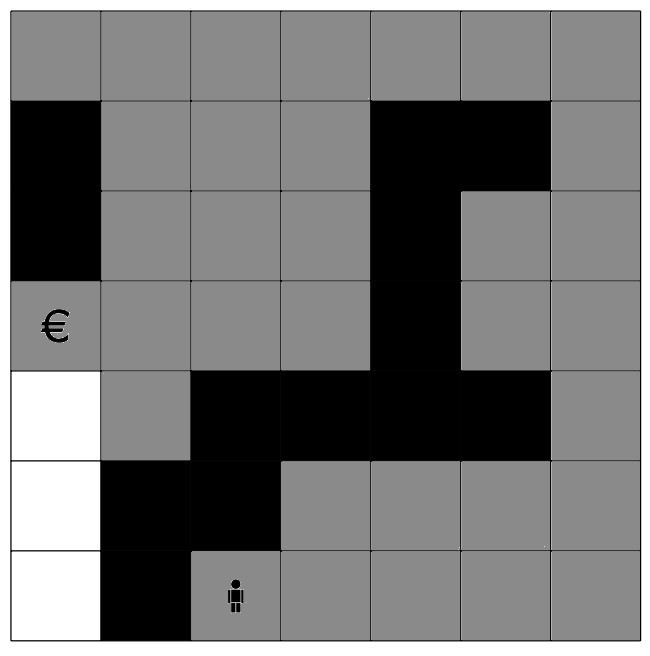
\includegraphics[scale=0.4]{uniform.JPG} 
 \caption{Maze solved with uniform-cost graph search}
 \label{fig:uniform}
\end{figure}


\subsection*{Show on the right maze the board positions visited by A* graph search with a manhattan distance heuristic (ignoring walls). A state is visited when it is selected in the fringe and expanded. When several states have the smallest path cost, this uniform-cost search visits them in the same lexicographical order as the one used for uniform-cost graph search.}

The figure \ref{fig:manhattan} shows the maze solved with the  A* graph search with a manhattan distance heuristic.

\begin{figure}[!ht] % ou [!ht] force ([!]) to insert image here ([h]ere) or on the top of the page ([t]op)
 \centering
 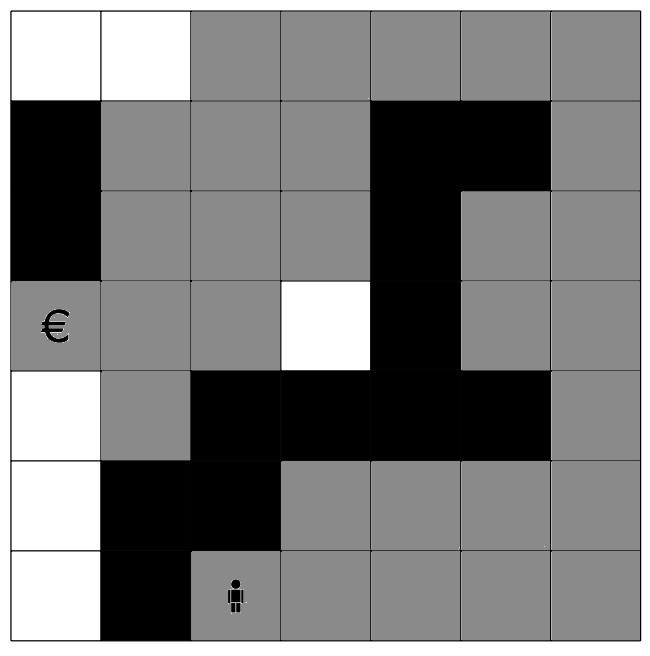
\includegraphics[scale=0.4]{manhattan.JPG} 
 \caption{Maze solved with A* graph search with a manhattan heuristic}
 \label{fig:manhattan}
\end{figure}

\newpage
\section{Sokoban problem}
\subsection*{As illustrated on Figure 3 some situations cannot lead to a solution. Are there other similar situations ? If yes, describe them.}

Yes, in addition to having a box in a corner, we have thoses situations:
\begin{itemize}
    \item A box with 2 adjacents walls (like a corner but anywhere in the grid) as showed in figure \ref{fig:dead1}
    \item A 2 by 2 square formed by either boxes or walls and boxes as showed in figure \ref{fig:dead2}
\end{itemize}

\begin{figure}[h] % ou [!ht] force ([!]) to insert image here ([h]ere) or on the top of the page ([t]op)
 \centering
 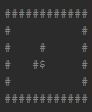
\includegraphics[scale=1.5]{dead1.JPG} 
 \caption{Dead state; \$ is a box, \# are walls}
 \label{fig:dead1}
\end{figure}

\begin{figure}[h] % ou [!ht] force ([!]) to insert image here ([h]ere) or on the top of the page ([t]op)
 \centering
 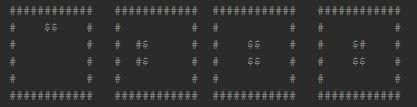
\includegraphics[width=\textwidth]{dead2.JPG} 
 \caption{Dead state}
 \label{fig:dead2}
\end{figure}

\subsection*{Why is it important to identify dead states in your successor function ? How you going to implement it ?}
It is important because if we didn't perform dead states detection, the algorithm is going to explore a lot of other states trying to reach the goal before realizing that there is no solution. So it saves time and memory.

To implement this function, we need to know which box had just been moved. Because if they weren't dead states before a move, the only position where a dead state can append is at the position where the box has moved (and of course if no box was moved, there is no dead state).
Then, we check if the box is near 2 walls. The different cases we check are:
\begin{itemize}
\item Is there a wall UP and LEFT (see figure \ref{fig:dead1})
\item Is there a wall UP and RIGHT
\item Is there a wall DOWN and LEFT
\item Is there a wall DOWN and RIGHT
\end{itemize}
As soon as one of the previous case occurs, we can say that there is a dead state with the moved box.
Actually, checking those cases include the dead state example included in the statement paper.

If no dead state was detect so far, we are going to check the 4 possible 2 by 2 squares containing the moved box.
For each 2 by 2 square, we check the 3 positions adjacent to the box. If they all are boxes or walls, we detect a dead state (see figure \ref{fig:dead2})

\subsection*{Describe possible (non trivial) heuristic(s) to reach a goal state (with reference if any). Is(are) your heuristic(s) admissible and/or consistent ?}

\subsubsection*{Heuristic 1}
A possible heuristic is to addition for all the blocks the manhattan distance between the block and the closest free target from it. In addition we compute also the manhattan distance between the person and the closest block unplaced from him.


This heuristic h can be written as the following calculation :
h = a + b where :
\begin{itemize}
\item a : the sum of the manhattan distance between each block and its closest free target.
\item b : the manhattan distance between the person and the closer block unplaced
\end{itemize}

This heuristic is admissible because :
\begin{itemize}
\item{$a + b \ge 0 $}\\
As a is an addition of manhattan distances and b is a manhattan distance then $a + b$ is always greater than or equal to 0.
\item{$a + b \le $ minimum possible distance to be covered}\\
This distance can be written as $a^{'} + b^{'}$ where $a^{'}$ is the addition of the shorter path between all the blocks and the closest free target from them. $b^{'}$ is the shorter path between the player and the closest block from him.
\begin{itemize}
\item{$a \le a^{'}$}: a is a sum between manhattan distances. By definition a is always the minimum distance.
\item{$b \le b^{'}$}: b is a manhattan distance then by definition it is always the minimum distance.
\end{itemize}
So in conclusion, $a + b \ge 0 $ then this heuristic is admissible. 
\end{itemize}
This heuristic is consistent because :\\
According to the course, we need to prove $h(n) \le c(n,a,n^{'}) + h(n^{'})$. The estimated cost of reaching the goal from n is no greater than the step cost of getting to $n^{'}$ plus the estimated cost of reaching the goal from $n^{'}$.

Trivially, $h(n)$ and $h(n^{'})$ are heuristics calculated by manhattan distances so they are the minimal distance to travel to reach the goal. Then $c(n,a,n^{'})$ is either the shortest path between $n$ and $n'$ or it's a longer path between this two points. So we can say that in the best case $h(n) = c(n,a,n^{'}) + h(n^{'})$ and in other cases $h(n) \le c(n,a,n^{'}) + h(n^{'})$. We can conclude that our heuristic is consistent.

\subsection*{Experiment, compare, analyze informed (astar\_graph\_search) and uninformed (breadth\_first\_graph\_search) graph search of aima-python3 on the 5 instances of sokoban provided. Report in a table the time, the number of explored nodes and the number of steps to reach the solution. Are the number of explored nodes always smaller with astar\_graph\_search, why ?
When no solution can be found by a strategy in a reasonable time (say 5 min), explain the reason (time-out and/or swap of memory)}

As we can see in the table 1, the A* graph search always explore less nodes than the Uninformed graph search. This can be explained because with Uniformed graph search there is no heuristic function that choose the best way to reach the solution, so the search is less efficient.
For the most difficult instance (sokoInst15), we can see that the A* graph search is 4 time faster and explore 14 time less nodes to reach the solution.
Howhever, our algorithm was able to find a solution for each instance in a reasonable time, even using the Uninformed graph search.

\begin{table}
\centering
\label{tab:results}
\begin{tabular}{c|c|c|c|c|c|c|}
 & \multicolumn{3}{c|}{A* graph search} & \multicolumn{3}{c}{Uninformed graph search} & 
 \hline
Instance Name & Time & Nodes explored & Steps & Time & Nodes explored & Steps \\
\hline
sokoInst01 & 0,191128969 &	1506 &	14 & 0,492327929 & 3825 & 14 \\
sokoInst02 & 1,092726946 &	5772 &	64 & 4,853234053 & 30541 & 64 \\
sokoInst07 & 0,743494034 &	3500 &	97 & 2,081387043 & 9522 & 97 \\
sokoInst08 & 0,98766017  &	4449 &	89 & 3,018009901 & 13649 & 89 \\
sokoInst15 & 14,65776491 &	60583 &	55 & 165,761421 & 810820 & 55 \\


\end{tabular}
\caption{Results of the 4 settings running on the 9 instances}

\end{table}


\subsection*{What are the performances of your program when you don't perform dead state detection ?}

Without dead state detection, the program take up to 14 more time to solve the problem and explore up to 12 more nodes.
The figure \ref{dia:sec} shows the difference of time to solve the instance with and without dead state detection.
The figure \ref{dia:nodes} shows the difference of nodes explored to solve the instance with and without dead state detection.
The number of steps to reach the solution is the same with and without dead state detection so we didn't produce a graph to compare them.

\begin{figure}[h] % ou [!ht] force ([!]) to insert image here ([h]ere) or on the top of the page ([t]op)
 \centering
 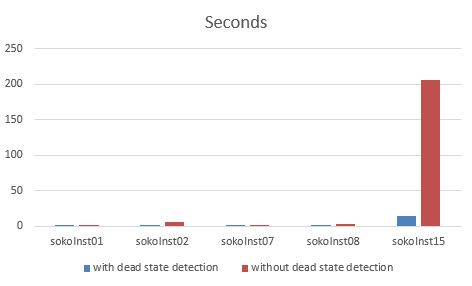
\includegraphics[scale=0.9]{seconds.JPG} 
 \caption{Comparaison of the seconds to solve instances with and without dead state detection}
 \label{dia:sec}
\end{figure}

\begin{figure}[h] % ou [!ht] force ([!]) to insert image here ([h]ere) or on the top of the page ([t]op)
 \centering
 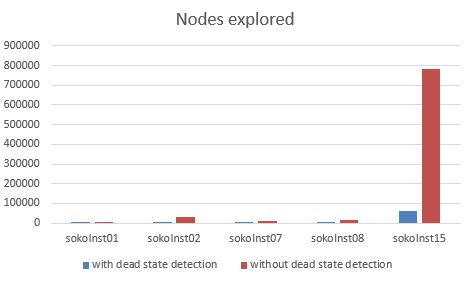
\includegraphics[scale=0.9]{nodes.JPG} 
 \caption{Comparaison of the nodes explored to solve instances with and without dead state detection}
 \label{dia:nodes}
\end{figure}




\end{document}
